\section{The one-bit frontier}
\label{sec:onebit}

The smallest interesting record keeps a single bit. Here the frontier is exact,
closed-form, and---perhaps surprisingly---\emph{linear} in the required margin.

\begin{theorem}[One-bit frontier]
\label{thm:onebit}
Let $n$ be odd, $S$ uniform on $\cube$, $K = 2$, with arbitrary bounded payment
decoders and arbitrary reconstruction. Put
\[
  \Mn \;=\; 2^{-n}\sum_{k=0}^{n}\binom{n}{k}\min(k,\,n-k)
       \;=\; \E\bigl[\min(|S|, n-|S|)\bigr].
\]
Then for $0 \le \gamma \le 1/n$,
\[
  \Dopt(2,\gamma) \;=\; \Mn + n\gamma\Bigl(\tfrac{n-1}{2} - \Mn\Bigr),
\]
and no record implements margin $\gamma > 1/n$ at all, whatever the payment.
\end{theorem}

\paragraph{Why it is linear.}
For $K = 2$ the record is a single function $\enc : \cube \to [0,1]$, and the
margin condition factors into a per-agent orientation. Aligning the orientations
by input flips --- valid precisely because the uniform prior is flip-invariant
and Hamming loss flip-equivariant --- turns the feasible set into an affine shift
of the monotone cone, on which the objective is linear for a fixed reconstruction
pair. A linear objective on a shifted cone is what produces a straight frontier
rather than a curved one. The optimal record is a mixture of two classical
objects, \emph{majority} and a \emph{random-bit sampler}; neither is new, and the
content of Theorem~\ref{thm:onebit} is that nothing else does better.
Appendix~\ref{app:onebit} carries the derivation in full.

\paragraph{Order of argument (this matters).}
Under \emph{optimal} decoding, $D(\enc)$ is a minimum of linear functionals and
hence \emph{concave} in $\enc$, so permutation-averaging can only
\emph{increase} it: a symmetrisation applied before the decoder is fixed runs
the wrong way for a lower bound. The correct order, used above and in
Appendix~\ref{app:onebit}, is: fix the reconstruction pair, for which the
objective is linear in $\enc$; optimise over $\enc$; and only then minimise over
reconstruction pairs.

That last step is carried out for general~$n$ in
Proposition~\ref{prop:antipodal}. Write $\Delta_{a,b}(s) = \dH(s,b) - \dH(s,a)$
and split the coordinates of the pair into the $p$ positions with
$(a_i,b_i) = (0,1)$ and the $m$ with $(1,0)$. The term of the objective that the
record can still influence is controlled by $\E[\Delta_{a,b}(S)^-]$, and that
quantity equals $\tfrac12 \E|R_{p+m}|$, where $R_k$ is a sum of $k$ independent
Rademacher variables. Since $\E|R_k|$ is nondecreasing in $k$ and $p + m \le n$,
every pair is dominated by the antipodal one, where $p = n$. The proof needs no
averaging step and no orbit enumeration; the reduction of pairs under $S_n$ to
the $\binom{n+3}{3}$ orbits indexed by $(n_{00},n_{01},n_{10},n_{11})$ is used
only to verify it.

\paragraph{Verification.}
Table~\ref{tab:onebit} reports an independent check: for each $n$ and each
$\gamma$ on a grid spanning $[0, 1/n]$, an LP over $\enc$ for every
reconstruction orbit, compared against the closed form. The orbit reduction was
itself cross-checked against complete enumeration of all $4^n$ pairs at $n = 3$
and $n = 5$ (agreement to $0$), and orientation invariance was confirmed across
all eight sign patterns at $n = 3$ (spread $0$). In every case the optimiser
landed exactly on the conjectured record
$\enc(s) = \gamma|s| + (1-n\gamma)\ind{|s| > n/2}$.

\begin{table}[t]
\centering
\caption{Theorem~\ref{thm:onebit} against exhaustive-orbit LP.
Recomputed in the pinned environment (Python 3.10.11, NumPy 2.2.6,
SciPy 1.15.3).}
\label{tab:onebit}
\begin{tabular}{@{}lrrr@{}}
\toprule
$n$ & $\Mn$ & $\gamma$ range & max deviation \\
\midrule
3 & 0.750000 & $[0, 1/3]$ & $0$ \\
5 & 1.562500 & $[0, 1/5]$ & $0$ \\
7 & 2.406250 & $[0, 1/7]$ & $4.4\times10^{-16}$ \\
9 & 3.269531 & $[0, 1/9]$ & $3.1\times10^{-15}$ \\
\bottomrule
\end{tabular}
\end{table}

\begin{figure}[t]
\centering
% Generated by make_figures.py -- do not edit by hand.
% Requires \usepackage{pgfplots} in the preamble.
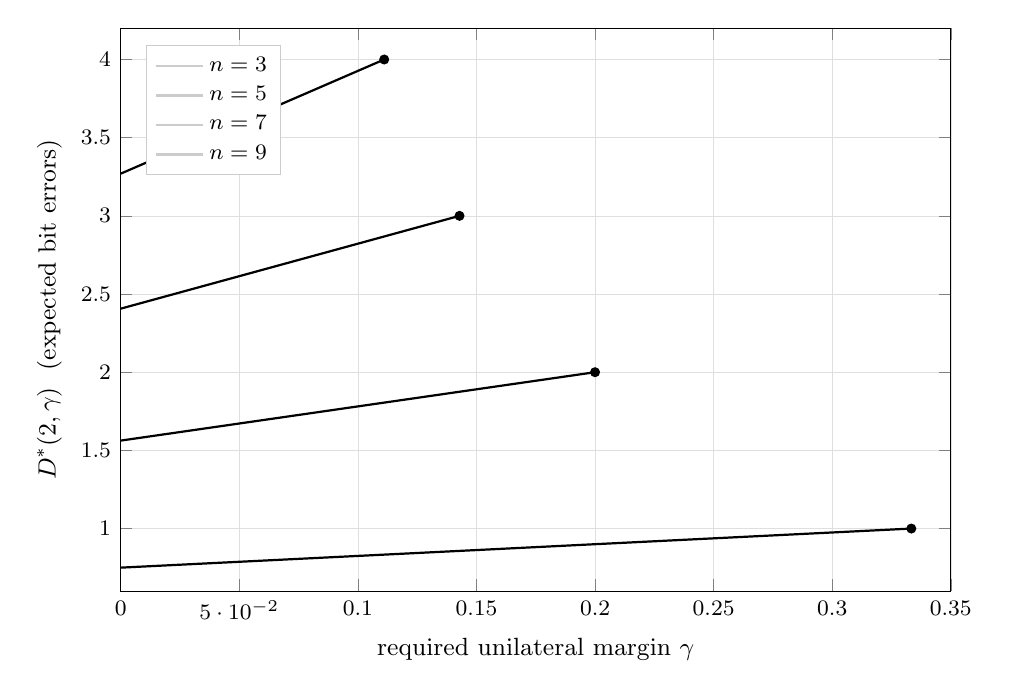
\begin{tikzpicture}
\begin{axis}[
  width=\columnwidth, height=0.72\columnwidth,
  xlabel={required unilateral margin $\gamma$},
  ylabel={$D^\ast(2,\gamma)$ \ (expected bit errors)},
  xmin=0, xmax=0.35, ymin=0.6, ymax=4.2,
  legend pos=north west, legend cell align=left,
  grid=major, grid style={very thin, gray!25},
  tick label style={font=\footnotesize},
  label style={font=\small},
  legend style={font=\footnotesize, draw=gray!40},
]
\addplot[thick] coordinates {(0.000000,0.750000) (0.008333,0.756250) (0.016667,0.762500) (0.025000,0.768750) (0.033333,0.775000) (0.041667,0.781250) (0.050000,0.787500) (0.058333,0.793750) (0.066667,0.800000) (0.075000,0.806250) (0.083333,0.812500) (0.091667,0.818750) (0.100000,0.825000) (0.108333,0.831250) (0.116667,0.837500) (0.125000,0.843750) (0.133333,0.850000) (0.141667,0.856250) (0.150000,0.862500) (0.158333,0.868750) (0.166667,0.875000) (0.175000,0.881250) (0.183333,0.887500) (0.191667,0.893750) (0.200000,0.900000) (0.208333,0.906250) (0.216667,0.912500) (0.225000,0.918750) (0.233333,0.925000) (0.241667,0.931250) (0.250000,0.937500) (0.258333,0.943750) (0.266667,0.950000) (0.275000,0.956250) (0.283333,0.962500) (0.291667,0.968750) (0.300000,0.975000) (0.308333,0.981250) (0.316667,0.987500) (0.325000,0.993750) (0.333333,1.000000)};
\addlegendentry{$n=3$}
\addplot[only marks, mark=*, mark size=1.6pt, forget plot] coordinates {(0.333333,1.000000)};
\addplot[thick] coordinates {(0.000000,1.562500) (0.005000,1.573438) (0.010000,1.584375) (0.015000,1.595312) (0.020000,1.606250) (0.025000,1.617188) (0.030000,1.628125) (0.035000,1.639063) (0.040000,1.650000) (0.045000,1.660937) (0.050000,1.671875) (0.055000,1.682813) (0.060000,1.693750) (0.065000,1.704687) (0.070000,1.715625) (0.075000,1.726562) (0.080000,1.737500) (0.085000,1.748438) (0.090000,1.759375) (0.095000,1.770312) (0.100000,1.781250) (0.105000,1.792188) (0.110000,1.803125) (0.115000,1.814062) (0.120000,1.825000) (0.125000,1.835938) (0.130000,1.846875) (0.135000,1.857813) (0.140000,1.868750) (0.145000,1.879688) (0.150000,1.890625) (0.155000,1.901563) (0.160000,1.912500) (0.165000,1.923437) (0.170000,1.934375) (0.175000,1.945312) (0.180000,1.956250) (0.185000,1.967188) (0.190000,1.978125) (0.195000,1.989063) (0.200000,2.000000)};
\addlegendentry{$n=5$}
\addplot[only marks, mark=*, mark size=1.6pt, forget plot] coordinates {(0.200000,2.000000)};
\addplot[thick] coordinates {(0.000000,2.406250) (0.003571,2.421094) (0.007143,2.435938) (0.010714,2.450781) (0.014286,2.465625) (0.017857,2.480469) (0.021429,2.495312) (0.025000,2.510156) (0.028571,2.525000) (0.032143,2.539844) (0.035714,2.554688) (0.039286,2.569531) (0.042857,2.584375) (0.046429,2.599219) (0.050000,2.614063) (0.053571,2.628906) (0.057143,2.643750) (0.060714,2.658594) (0.064286,2.673437) (0.067857,2.688281) (0.071429,2.703125) (0.075000,2.717969) (0.078571,2.732813) (0.082143,2.747656) (0.085714,2.762500) (0.089286,2.777344) (0.092857,2.792187) (0.096429,2.807031) (0.100000,2.821875) (0.103571,2.836719) (0.107143,2.851562) (0.110714,2.866406) (0.114286,2.881250) (0.117857,2.896094) (0.121429,2.910938) (0.125000,2.925781) (0.128571,2.940625) (0.132143,2.955469) (0.135714,2.970312) (0.139286,2.985156) (0.142857,3.000000)};
\addlegendentry{$n=7$}
\addplot[only marks, mark=*, mark size=1.6pt, forget plot] coordinates {(0.142857,3.000000)};
\addplot[thick] coordinates {(0.000000,3.269531) (0.002778,3.287793) (0.005556,3.306055) (0.008333,3.324316) (0.011111,3.342578) (0.013889,3.360840) (0.016667,3.379102) (0.019444,3.397363) (0.022222,3.415625) (0.025000,3.433887) (0.027778,3.452148) (0.030556,3.470410) (0.033333,3.488672) (0.036111,3.506934) (0.038889,3.525195) (0.041667,3.543457) (0.044444,3.561719) (0.047222,3.579980) (0.050000,3.598242) (0.052778,3.616504) (0.055556,3.634766) (0.058333,3.653027) (0.061111,3.671289) (0.063889,3.689551) (0.066667,3.707813) (0.069444,3.726074) (0.072222,3.744336) (0.075000,3.762598) (0.077778,3.780859) (0.080556,3.799121) (0.083333,3.817383) (0.086111,3.835645) (0.088889,3.853906) (0.091667,3.872168) (0.094444,3.890430) (0.097222,3.908691) (0.100000,3.926953) (0.102778,3.945215) (0.105556,3.963477) (0.108333,3.981738) (0.111111,4.000000)};
\addlegendentry{$n=9$}
\addplot[only marks, mark=*, mark size=1.6pt, forget plot] coordinates {(0.111111,4.000000)};
\end{axis}
\end{tikzpicture}

\caption{The exact one-bit frontier. Each line is
Theorem~\ref{thm:onebit} over its whole admissible range and terminates at the
marked point $(1/n,\,(n-1)/2)$, beyond which no record implements the required
margin. Generated from the closed form by \texttt{make\_figures.py}.}
\label{fig:frontier}
\end{figure}

\begin{remark}[Endpoint]
\label{rem:endpoint}
Substituting $\gamma = 1/n$ collapses the formula to $\Dopt(2,1/n) = (n-1)/2$,
independently of $\Mn$: at the maximum implementable margin the record is worth
exactly half a bit per agent less than guessing, whatever $n$ is. The frontier therefore runs from $(0,\Mn)$ to $(1/n,(n-1)/2)$ and is
determined by its endpoints; Figure~\ref{fig:frontier} plots it for
$n = 3,5,7,9$.
\end{remark}
